\begin{enumerate}[label=\thesubsection.\arabic*, ref=\thesubsection.\theenumi]
%
\item For the AP 
$$\frac{3}{2}, \frac{1}{2}, -\frac{1}{2}, -\frac{3}{2}, \dots $$ write the first term $a$ and the common difference $d$.
\item Which of the following list of numbers form an AP? If they form an AP, 
write the next two terms 
		\begin{multicols}{2}
\begin{enumerate}
\item $4, 10, 16, 22, \dots$ 
\item $1, -1, -3, -5, \dots$ 
\item $-2, 2, -2, 2, -2, \dots$
\item $1, 1, 1, 2, 2, 2, 3, 3, 3, \dots$
\end{enumerate}
\end{multicols}
\item Find the 10th term of the AP : $2,  7,  12,  \dots$
\item Which term of the AP : $21,  18,  15,  \dots$ is - 81? Also,  is any term 0? Give reason for your answer.
\item Determine the AP whose 3rd term is 5 and the 7th term is 9.
\item Check whether 301 is a term of the list of numbers $5,  11,  17,  23,  \dots$
\item How many two-digit numbers are divisible by 3?
\item Find the 11th term from the last term (towards the first term) of the
AP : $10,  7,  4,  \dots,  - 62$.
\item A sum of \rupee 1000 is invested at $8\%$ simple interest per year. Calculate the interest at the end of each year. Do these interests form an AP? If so,  find the interest at the end of 30 years making use of this fact.
\item In a flower bed,  there are 23 rose plants in the first row,  21 in the
second,  19 in the third,  and so on. There are 5 rose plants in the last row. How many rows are there in the flower bed?
\item Find the sum of the first 22 terms of the AP : $8,  3,  -2,  \dots$
\item If the sum of the first 14 terms of an AP is 1050 and its first term is 10,  find the 20th term.
\item How many terms of the AP : $24,  21,  18,  \dots$ must be taken so that their
sum is 78?
\item Find the sum of 
\begin{enumerate}
\item the first 1000 positive integers.
\item the first $n$ positive integers.
\end{enumerate}
\item Find the sum of first 24 terms of the list of numbers whose $n^{th}$ term is given by $a_n = 3 + 2n$
\item A manufacturer of TV sets produced 600 sets in the third year and 700
sets in the seventh year. Assuming that the production increases uniformly by a fixed number every year,  find 
\begin{enumerate}
\item   the production in the 1st year
\item	the production in the 10th year
\item the total production in first 7 years.
\end{enumerate}
\item In which of the following situations,  does the list of numbers involved make an arithmetic progression,  and why?
\begin{enumerate}
\item The taxi fare after each km when the fare is \rupee 15 for the first km and \rupee 8 for each additional km.
\item The amount of air present in a cylinder when a vacuum pump removes 
$\frac{1}{4}$ of the air remaining in the cylinder at a time.
\item  The cost of digging a well after every metre of digging,  when it costs \rupee 150 for the first metre and rises by \rupee 50 for each subsequent metre.
\item The amount of money in the account every year,  when \rupee 10000 is deposited at compound interest at 8 \% per annum.
\end{enumerate}
\item Write first four terms of the AP,  when the first term $a$ and the common difference $d$ are
given as follows
		\begin{multicols}{2}
\begin{enumerate}
\item $a = 10,  d = 10	$	
\item $a = 4,  d = -3	$	
\item $a = -2,  d = 0	$	
\item $ a = -1,  d =\frac{1}{2}$
\item $a = -1.25,  d = -0.25$	
\end{enumerate}
\end{multicols}
\item For the following APs,  write the first term and the common difference
	\begin{multicols}{2}
		\begin{enumerate}[itemsep=1ex]
\item $3,  1,  -1,  -3,  \dots $
\item $-5,  -1,  3,  7,  \dots $
\item $\frac{1}{3},  \frac{5}{3},  \frac{9}{3},  \frac{13}{3}, \dots $
\item $0.6,  1.7,  2.8,  3.9, \dots $ 
\end{enumerate}
\end{multicols}
\item Which of the following are APs? If they form an AP,  find the common difference $d$ and
write three more terms.
\begin{multicols}{2}
\begin{enumerate}[itemsep=1ex]
\item $2,  4,  8,  16,  \dots $
\item $2, \frac{5}{2},  3,  \frac{7}{2}, \dots $
\item $-1.2,  -3.2,  -5.2,  -7.2,  \dots $
\item $-10,  -6,  -2,  2,  \dots $
\item $3, 3+\sqrt{2},  3+2\sqrt{2},  3+3\sqrt{2}, \dots $
\item $0.2,  0.22,  0.222,  0.2222,  \dots $
\item $0,  -4,  -8,  -12,  \dots $
\item $-\frac{1}{2},  -\frac{1}{2},  -\frac{1}{2},  -\frac{1}{2}, \dots $
\item $1,  3,  9,  27, \dots $ 
\item $a,  2a,  3a,  4a, \dots $ 
\item $a,  a^2,  a^3,  a^4, \dots $
\item $\sqrt{2},  \sqrt{8},  \sqrt{18},  \sqrt{32}, \dots $
\item $\sqrt{3},  \sqrt{6},  \sqrt{9},  \sqrt{12}, \dots $
\item $1^2,  3^2,  5^2,  7^2, \dots$
\item $1^2,  5^2,  7^2,  73, \dots $
\end{enumerate}
\end{multicols}
\item Fill in the blanks in 
	\tabref{table:ap},  given that $a$ is the first term,  $d$ the common
difference and $a_n$ the $n^{th}$ term of the AP.
\begin{table}[H]
	\centering
\begin{tabular}{|c|c|r|l|l|}
\hline
\\
&$a$& $d$ & $n$ & $a_n$
\\
\hline
(i)& 	7 &3 &8 &$\dots $ 
\\
(ii)& 	-18 &$\dots $  &10  &0
\\
(iii)& 	$\dots $  &-3 &18 &-5
\\
(iv)& 	-18.9 &2.5 &$\dots $  &3.6
\\
(v)& 	3.5 &0 &105 &$\dots $ 
\\
\hline
\end{tabular}
	\caption{}
	\label{table:ap}
\end{table}
\item Choose the correct choice in the following and justify 
\begin{enumerate}
	\item $30^{th}$ term of the AP: $10,  7,  4, \dots $   is
	\begin{multicols}{4}
\begin{enumerate}
\item 97
\item 77
\item -77
\item -87
\end{enumerate}
\end{multicols}
\item $11^{th}$ term of the AP: $ -3,  -\frac{1}{2},  2, \dots  $ is 
	\begin{multicols}{4}
\begin{enumerate}
\item 28
\item 22
\item -38
\item $-48\frac{1}{2}$
\end{enumerate}
\end{multicols}
\item In the following APs,  find the missing terms in the blanks  
	\begin{multicols}{2}
\begin{enumerate}
\item $2,  \dots,  26$
\item $\dots  ,  13, \dots  ,  3$
\item $5,  \dots  ,  \dots  ,  9\frac{1}{2}$
\item $-4,  \dots  ,  \dots  ,  \dots  ,  \dots,  6$
\item $\dots ,  38,  \dots ,  \dots ,  \dots ,  -22$
\end{enumerate}
\end{multicols}
\end{enumerate}
\item Which term of the AP : $3,  8,  13,  18,  \dots $ is 78?
\item Find the number of terms in each of the following APs:
\begin{enumerate}
	\item $7,  13,  19,  \dots , 205$.
	\item $18,  15\frac{1}{2},  13, \dots , -47$
\end{enumerate}
\item Check whether -150 is a term of the AP : $11,  8,  5,  2 \dots $ 
\item Find the 31st term of an AP whose 11th term is 38 and the 16th term is 73.
\item An AP consists of 50 terms of which 3rd term is 12 and the last term is 106. Find the 29th term.
\item If the 3rd and the 9th terms of an AP are 4 and -8 respectively,  which term of this AP is zero?
\item The 17th term of an AP exceeds its 10th term by 7. Find the common difference.
\item Which term of the AP : $3,  15,  27,  39, \dots $  will be 132 more than its 54th term? 
\item How many three-digit numbers are divisible by 7?
\item How many multiples of 4 lie between 10 and 250?
\item For what value of $n$,  are the $n^{th}$ terms of two APs: $63,  65,  67, \dots $  and $3,  10,  17, \dots $  equal?
\item Determine the AP whose third term is 16 and the 7th term exceeds the 5th term by 12.
\item Find the 20th term from the last term of the AP : $3,  8,  13, \dots  ,  253$.
\item The sum of the 4th and 8th terms of an AP is 24 and the sum of the 6th and 10th terms is 44. Find the first three terms of the AP.
\item Subba Rao started work in 1995 at an annual salary of \rupee 5000 and received an increment of \rupee 200 each year. In which year did his income reach \rupee 7000?
\item Ramkali saved \rupee 5 in the first week of a year and then increased her weekly savings by \rupee 1.75. If in the $n^{th}$ week,  her weekly savings become \rupee 20.75,  find $n$.
\item Find the sum of the following APs
	\begin{multicols}{2}
\begin{enumerate}
	\item $2,  7,  12,  \dots $,  to 10 terms.
	\item $-37,  -33,  -29,  \dots $,  to 12 terms.
	\item $ 0.6,  1.7,  2.8,  \dots $,  to 100 terms.
	\item $\frac{1}{15},  \frac{1}{12},  \frac{1}{10}, \dots  $ to 11 terms.
\end{enumerate}
\end{multicols}
\item Find the sums given below 
\begin{enumerate}
\item $7+10\frac{1}{2}+14+\dots +84$
\item $34 + 32 + 30 + \dots + 10$
\item $-5 + (-8) + (-11) + \dots + (-230)$
\end{enumerate}
\item In an A.P
\begin{enumerate}
\item given $a = 5,  d = 3,  a_n = 50$,  find $n$ and $S_n$.
\item given $a = 7,  a_{13} = 35$,  find $d$ and $S_{13}$.
\item  given $a_{12} = 37,  d = 3$,  find $a$ and $S_{12}$.
\item given $a_3 = 15,  S_{10} = 125$,  find $d$ and $a_{10}$.
\item given $d = 5,  S_9= 75$,  find $a$ and $a_9$.
\item given $a = 2,  d = 8,  S_n = 90$,  find $n$ and $a_n$.
\item  given $a = 8,  a_n = 62,  S_n = 210$,  find $n$ and $d$.
\item given $a_n = 4,  d = 2,  S_n = -14$,  find $n$ and $a$.
\item given $a = 3,  n = 8,  S = 192$,  find $d$.
\item given $l = 28,  S = 144$,  and there are total 9 terms. Find $a$.
\end{enumerate}
\item How many terms of the AP : $9,  17,  25,  \dots $ must be taken to give a sum of 636?
\item The first term of an AP is 5,  the last term is 45 and the sum is 400. Find the number of terms and the common difference.
\item The first and the last terms of an AP are 17 and 350 respectively. If the common difference is 9,  how many terms are there and what is their sum?
\item Find the sum of first 22 terms of an AP in which d = 7 and 22nd term is 149.
\item Find the sum of first 51 terms of an AP whose second and third terms are 14 and 18 respectively.
\item If the sum of first 7 terms of an AP is 49 and that of 17 terms is 289,  find the sum of first $n$ terms. 
\item Show that $a_1 ,  a_2 ,  \dots,  a_n,  \dots$  form an AP where $a_n$ is defined as below 
\begin{enumerate}
	\item $a_n = 3 + 4n$
	\item $a_n = 9 - 5n$
\end{enumerate}
Also find the sum of the first 15 terms in each case.
\item If the sum of the first $n$ terms of an AP is $4n - n^2$,  what is the first term (that is $S_1$ )? What
is the sum of first two terms? What is the second term? Similarly,  find the 3rd,  the 10th and
the $n$th terms.
\item Find the sum of the first 40 positive integers divisible by 6.
\item Find the sum of the first 15 multiples of 8.
\item Find the sum of the odd numbers between 0 and 50.
\item A contract on construction job specifies a penalty for delay of completion beyond a
certain date as follows: \rupee 200 for the first day, \rupee 250 for the second day,  \rupee 300 for the third
day,  etc.,  the penalty for each succeeding day being \rupee 50 more than for the preceding day. How much money the contractor has to pay as penalty,  if he has delayed the work by 30 days?
\item A sum of \rupee 700 is to be used to give seven cash prizes to students of a school for their overall academic performance. If each prize is \rupee 20 less than its preceding prize,  find the value of each of the prizes.
\item  In a school,  students thought of planting trees in and around the school to reduce air pollution. It was decided that the number of trees,  that each section of each class will plant,  will be the same as the class,  in which they are studying,  
e.g.,  a section of Class I will plant 1 tree,  
a section of Class II will plant 2 trees and so on till Class XII. There are three sections of each class. How many trees will be planted by the students?
\item A spiral is made up of successive semicircles,  with centres alternately at A and B,  starting with centre at A,  of radii $0.5 cm,  1.0 cm,  1.5 cm,  2.0 cm, \dots $  as shown in Fig.
		\ref{fig:fig}
	What is the total length of such a spiral made up of thirteen consecutive 22 semicircles? (Take $\pi =\frac{22}{7}$)
	\begin{figure}[H]
		\centering
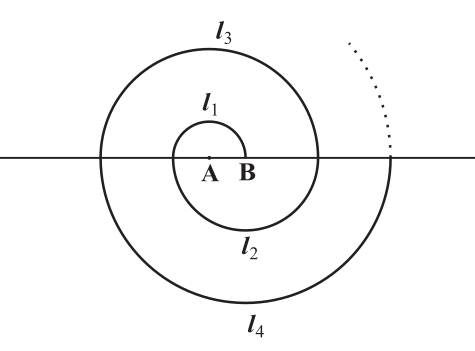
\includegraphics[width=0.75\columnwidth]{figs/ap/fig.png} 
		\caption{}
		\label{fig:fig}
	\end{figure}
{\em Hint:} Length of successive semicircles is $l_1,  l_2,  l_3,  l_4 ,  \dots$ with centres at A,  B,  A,  B,  $\dots $, respectively.
\item 200 logs are stacked in the following manner: 20 logs in the bottom row,  19 in the next row,  18 in the row next to it and so on (see Fig
		\ref{fig:fig1}
	). In how many rows are the 200 logs placed and how many logs are in the top row?
	\begin{figure}[H]
		\centering

\includegraphics[width=0.75\columnwidth]{figs/ap/fig1.png}
		\caption{}
		\label{fig:fig1}
	\end{figure}
\item In a potato race,  a bucket is placed at the starting point,  which is $5m$ from the first potato,  and the other potatoes are placed $3m$ apart in a straight line. There are ten potatoes in the line
		as shown in \figref{fig:fig3}.
	\begin{figure}[H]
		\centering
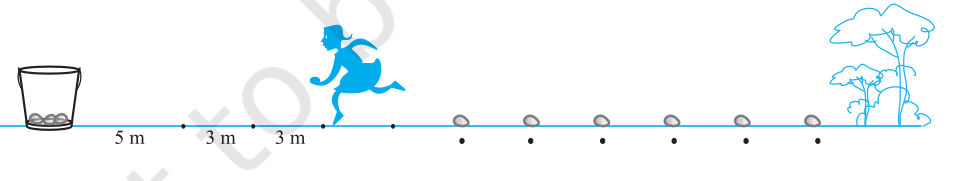
\includegraphics[width=0.75\columnwidth]{figs/ap/fig3.png} 
		\caption{}
		\label{fig:fig3}
	\end{figure}
A competitor starts from the bucket,  picks up the nearest potato,  runs back with it,  drops it in the bucket,  runs back to pick up the next potato,  runs to the bucket to drop it in,  and she continues in the same way until all the potatoes are in the bucket. What is the total distance the competitor has to run?\
[{\em Hint:} To pick up the first potato and the second potato,  the total distance (in metres)
run by a competitor is $2 \times 5 + 2 \times (5 + 3)$].
\item Which term of the AP : $121,  117,  113, \dots $ is its first negative term? [{\em Hint:} Find $n$ for $a_n < 0$]
\item The sum of the third and the seventh terms of an AP is 6 and their product is 8. Find the sum of first sixteen terms of the AP.
\item The houses of a row are numbered consecutively from 1 to 49. Show that there is a value of $x$ such that the sum of the numbers of the houses preceding the house numbered $x$ is equal to the sum of the numbers of the houses following it. Find this value of $x$.[{\em Hint:} $S_{x-1} = S_{49} -S_x$]
\item A small terrace at a football ground comprises of 15 steps each of which is $50 m$ long and built of solid concrete. Each step has rise of $\frac{1}{4}m$ and a tread of $\frac{1}{2}m$ 
	(see \figref{fig:fig5}).
	Calculate the total volume of concrete required to build the terrace. [{\em Hint:} Volume of concrete required to build the first step = $\frac{1}{4} \times \frac{1}{2} \times 50m^3$]
	\begin{figure}[H]
		\centering
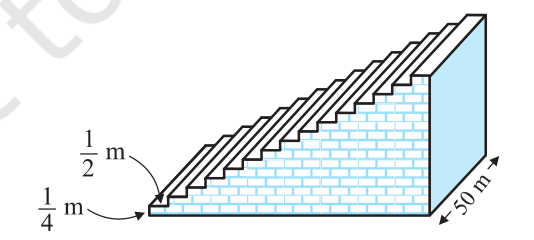
\includegraphics[width=0.75\columnwidth]{figs/ap/fig5.png}  
		\caption{}
		\label{fig:fig5}
	\end{figure}
\item Find the sum to $n$ terms of the following series
	\begin{multicols}{4}
\begin{enumerate}
	\item $a_n =2n+5$
	\item $a_n =\frac{n-3}{4}$
\item $a_n = \frac{2n-3}{6}$
\item $a_n = 4n-3 $
\end{enumerate}
\end{multicols}
\item Find the sum of all natural numbers lying between 100 and 1000,  which are multiples of 5.
\item In an AP,  the first term is 2 and the sum of the first five terms is one-fourth of the next five terms. Show that $20^{th}$ term is -112.
\item How many terms of the AP  $-6, -\frac{11}{2},  -5, \dots $ are needed to give the sum -25?
\item In an AP,  If $p^{th}$ term is $\frac{1}{q}, q^{th}$ term is $\frac{1}{p}$,  prove that the sum of first $pq$ terms is $\frac{1}{2}(pq+1)$,  where $p \neq q.$
\item  If the sum of a certain number of terms of the AP: $25,  22,  19,  \dots $  is 116, find the last term.
\item Find the sum to $n$ terms of the AP,  whose $k^{th}$ term is $5k + 1$.
\item If the sum of $n$ terms of an AP is $pn + qn^2$,  where $p$ and $q$ are constants,  find the common difference.
\item The sums of $n$ terms of two arithmetic progressions are in the ratio $5n + 4 : 9n + 6$. Find the ratio of their $18^{th}$ terms.
\item If the sum of first $p$ terms of an AP is equal to the sum of the first $q$ terms,  then find the sum of the first $p + q$ terms.
\item Sum of the first $p,  q$ and $r$ terms of an AP are $a,  b$ and $c$,  respectively. Prove that
$$\frac{a}{p}(q-r)+\frac{b}{q}(r-p)+\frac{c}{r}(p-q) = 0$$
\item The ratio of the sums of $m$ and $n$ terms of an AP is $m^2 : n^2$. Show that the ratio of 
$m^{th}$ and $n^{th}$ term is $(2m - 1) : (2n - 1)$.
\item If the sum of $n$ terms of an AP is $3n^2 + 5n$ and its $m^{th}$ term is 164,  find the value
of $m$.
\item Insert five numbers between 8 and 26 such that the resulting sequence is an AP
\item Between 1 and 31,  $m$ numbers have been inserted in such a way that the resulting sequence is an AP and the ratio of $7^{th}$ and $(m - 1)^{th}$ numbers is 5 : 9. Find the value of $m$.
\item A man starts repaying a loan as first instalment of \rupee 100. If he increases the
instalment by Rs 5 every month,  what amount he will pay in the $30^{th}$ instalment?
\item The difference between any two consecutive interior angles of a polygon is 5$\degree$. If the smallest angle is 120$\degree$,  find the number of the sides of the polygon. 
\item Show that the sum of $(m + n)^{th}$ and $(m - n)^{th}$ terms of an AP is equal to twice the $m^{th}$ term.
\item If the sum of three numbers in AP  is 24 and their product is 440,  find the numbers.
\item Let the sum of $n,  2n,  3n$ terms of an AP be $S_1,  S_2$ and $S_3$,  respectively,  show that 
$$S_3 = 3(S_2 - S_1)$$
\item Find the sum of all numbers between 200 and 400 which are divisible by 7.
\item Find the sum of integers from 1 to 100 that are divisible by 2 or 5.
\item  The sum of the first four terms of an AP  is 56. The sum of the last four terms is 112. If its first term is 11, then find the number of terms.
\item The $p^{th}, q^{th}$ and $r^{th}$ terms of an AP  are $a, b, c,$ respectively. Show that 
$$\brak{q - r }a + \brak{r - p }b + \brak{p - q }c = 0.$$
\item If $$a\brak{\frac{1}{b}+\frac{1}{c}}, b\brak{\frac{1}{c}+\frac{1}{a}}, c\brak{\frac{1}{a}+\frac{1}{b}}$$ are in AP, prove that $a, b, c$ are in AP. 
\item In an AP if the $m^{th}$ is $n$ and the $n^{th}$ term is $m$, where $m \ne n$, find the $p^{th}$ term.
\item If the sum of $n$ terms of an AP is
	$$nP+\frac{1}{2} n\brak{n-1}Q,$$
	where $P$ and $Q$ are constants, find the common difference.
\item The sum of $n$ terms of two arithmetic progressions are in the ratio
	$\brak{3n+8}:\brak{7n+15}$.  Find the ratio of their $12^{th}$ terms.
\item The income of a person is \rupee 3,00,000 in the first year and he receives an increase of \rupee 10,000 to his income per year for the next 19 years.  Find the total amount he received in 20 years.
\item Insert 6 numbers between 3 and 24 such that the resulting sequence is an AP.
\item Two APs have the same common difference. The difference between their 100th terms is 100,  what is the difference between their 1000th terms?
\item Find the sum of odd integers from 1 to 2001.
\item If $\frac{a^n+b^n}{a^{n-1}+b^{n-1}}$ is the AM  between $a$ and $b$,  then find the value of $n$.
\item Find the sum of all two digit numbers which when divided by 4,  yields 1 as remainder.
\item A farmer buys a used tractor for Rs 12000. He pays Rs 6000 cash and agrees to pay the balance in annual instalments of Rs 500 plus 12\% interest on the unpaid amount. How much will the tractor cost him?
\item Shyam Anand buys a scooter for Rs 22000. He pays Rs 4000 cash and agrees to
pay the balance in annual instalment of Rs 1000 plus 10\% interest on the unpaid
amount. How much will the scooter cost him?
\item A man deposited Rs 10000 in a bank at the rate of 5\% simple interest annually. Find the amount in the $15^{th}$ year since he deposited the amount and also calculate the total amount after 20 years.

\end{enumerate}
